\documentclass[10pt,twocolumn,letterpaper]{article}

\usepackage{cvpr}
\usepackage{times}
\usepackage{epsfig}
\usepackage{graphicx}
\usepackage{amsmath}
\usepackage{amssymb}

% Include other packages here, before hyperref.

% If you comment hyperref and then uncomment it, you should delete
% egpaper.aux before re-running latex.  (Or just hit 'q' on the first latex
% run, let it finish, and you should be clear).
\usepackage[breaklinks=true,bookmarks=false]{hyperref}

\cvprfinalcopy % *** Uncomment this line for the final submission

\def\cvprPaperID{****} % *** Enter the CVPR Paper ID here
\def\httilde{\mbox{\tt\raisebox{-.5ex}{\symbol{126}}}}

% Pages are numbered in submission mode, and unnumbered in camera-ready
%\ifcvprfinal\pagestyle{empty}\fi
\setcounter{page}{4321}
\begin{document}

%%%%%%%%% TITLE
\title{Dynamic Locomotion Terrain Recognition for the MIT Cheetah 3 Robot \\ 6.869 / 6.819: Advances in Computer Vision}

\author{Gerardo Bledt\\
Massachusetts Institute of Technology\\
Cambridge, MA\\
{\tt\small gbledt@mit.edu, 6.869}
% For a paper whose authors are all at the same institution,
% omit the following lines up until the closing ``}''.
% Additional authors and addresses can be added with ``\and'',
% just like the second author.
% To save space, use either the email address or home page, not both
\and
Milo Knowles\\
Massachusetts Institute of Technology\\
Cambridge, MA\\
{\tt\small mknowles@mit.edu, 6.819}
}

\maketitle
%\thispagestyle{empty}

%%%%%%%%% ABSTRACT
\begin{abstract}
   ADD ABSTRACT
\end{abstract}

%%%%%%%%% BODY TEXT

%!TEX root = ../egpaper_final.tex

\section{Introduction}

Currently, the MIT Cheetah 3 robot uses primarily completely blind locomotion. What this means is that there is no vision or LiDAR system that allows it to preemptively sense its environment or plan for upcoming obstacles. Dynamic gaits such as trotting have been stabilized under ideal flat-terrain conditions, but most interesting applications of robotics involve some kind of unstructured, non-flat, non-smooth terrain situations. Recent research efforts have allowed for reactive tactile environment sensing where the robot is able to interpret and build its knowledge of the environment when it senses unexpected contact with a surface \cite{Bledt2018}. This has allowed for the same nominal dynamic gaits to stabilize in rough terrains by reacting to the estimated foot contacts. 

However, since this environment sensing is purely reactionary, the robot can only detect objects and uneven ground after it has already determined contact with the surface. This covers a lot of cases where small objects and holes are littered over terrain with a slowly changing gradient. A current challenge is when the robot encounters a large, sharp terrain disturbances, such as a box or a set of stairs, it will not be able to smoothly use this reactionary sensing to navigate the terrain. If the box or stair is higher than the nominal foot swinging height as it is in Figure \ref{fig:RI}, it will simply not be able to step over it and will not detect a support surface contact when it does hit the side. Similarly, if the box or stair is higher than its possible foot swing height, it will not be able to continue forward and crash. By incorporating some visual terrain recognition, the robot will be able to modify its swing foot trajectory to clear objects that are within its kinematic workspace, as well as feed terrain information to the contact detection algorithm for more accurate probabilistic ground height models.

\begin{figure}[t]
\centering
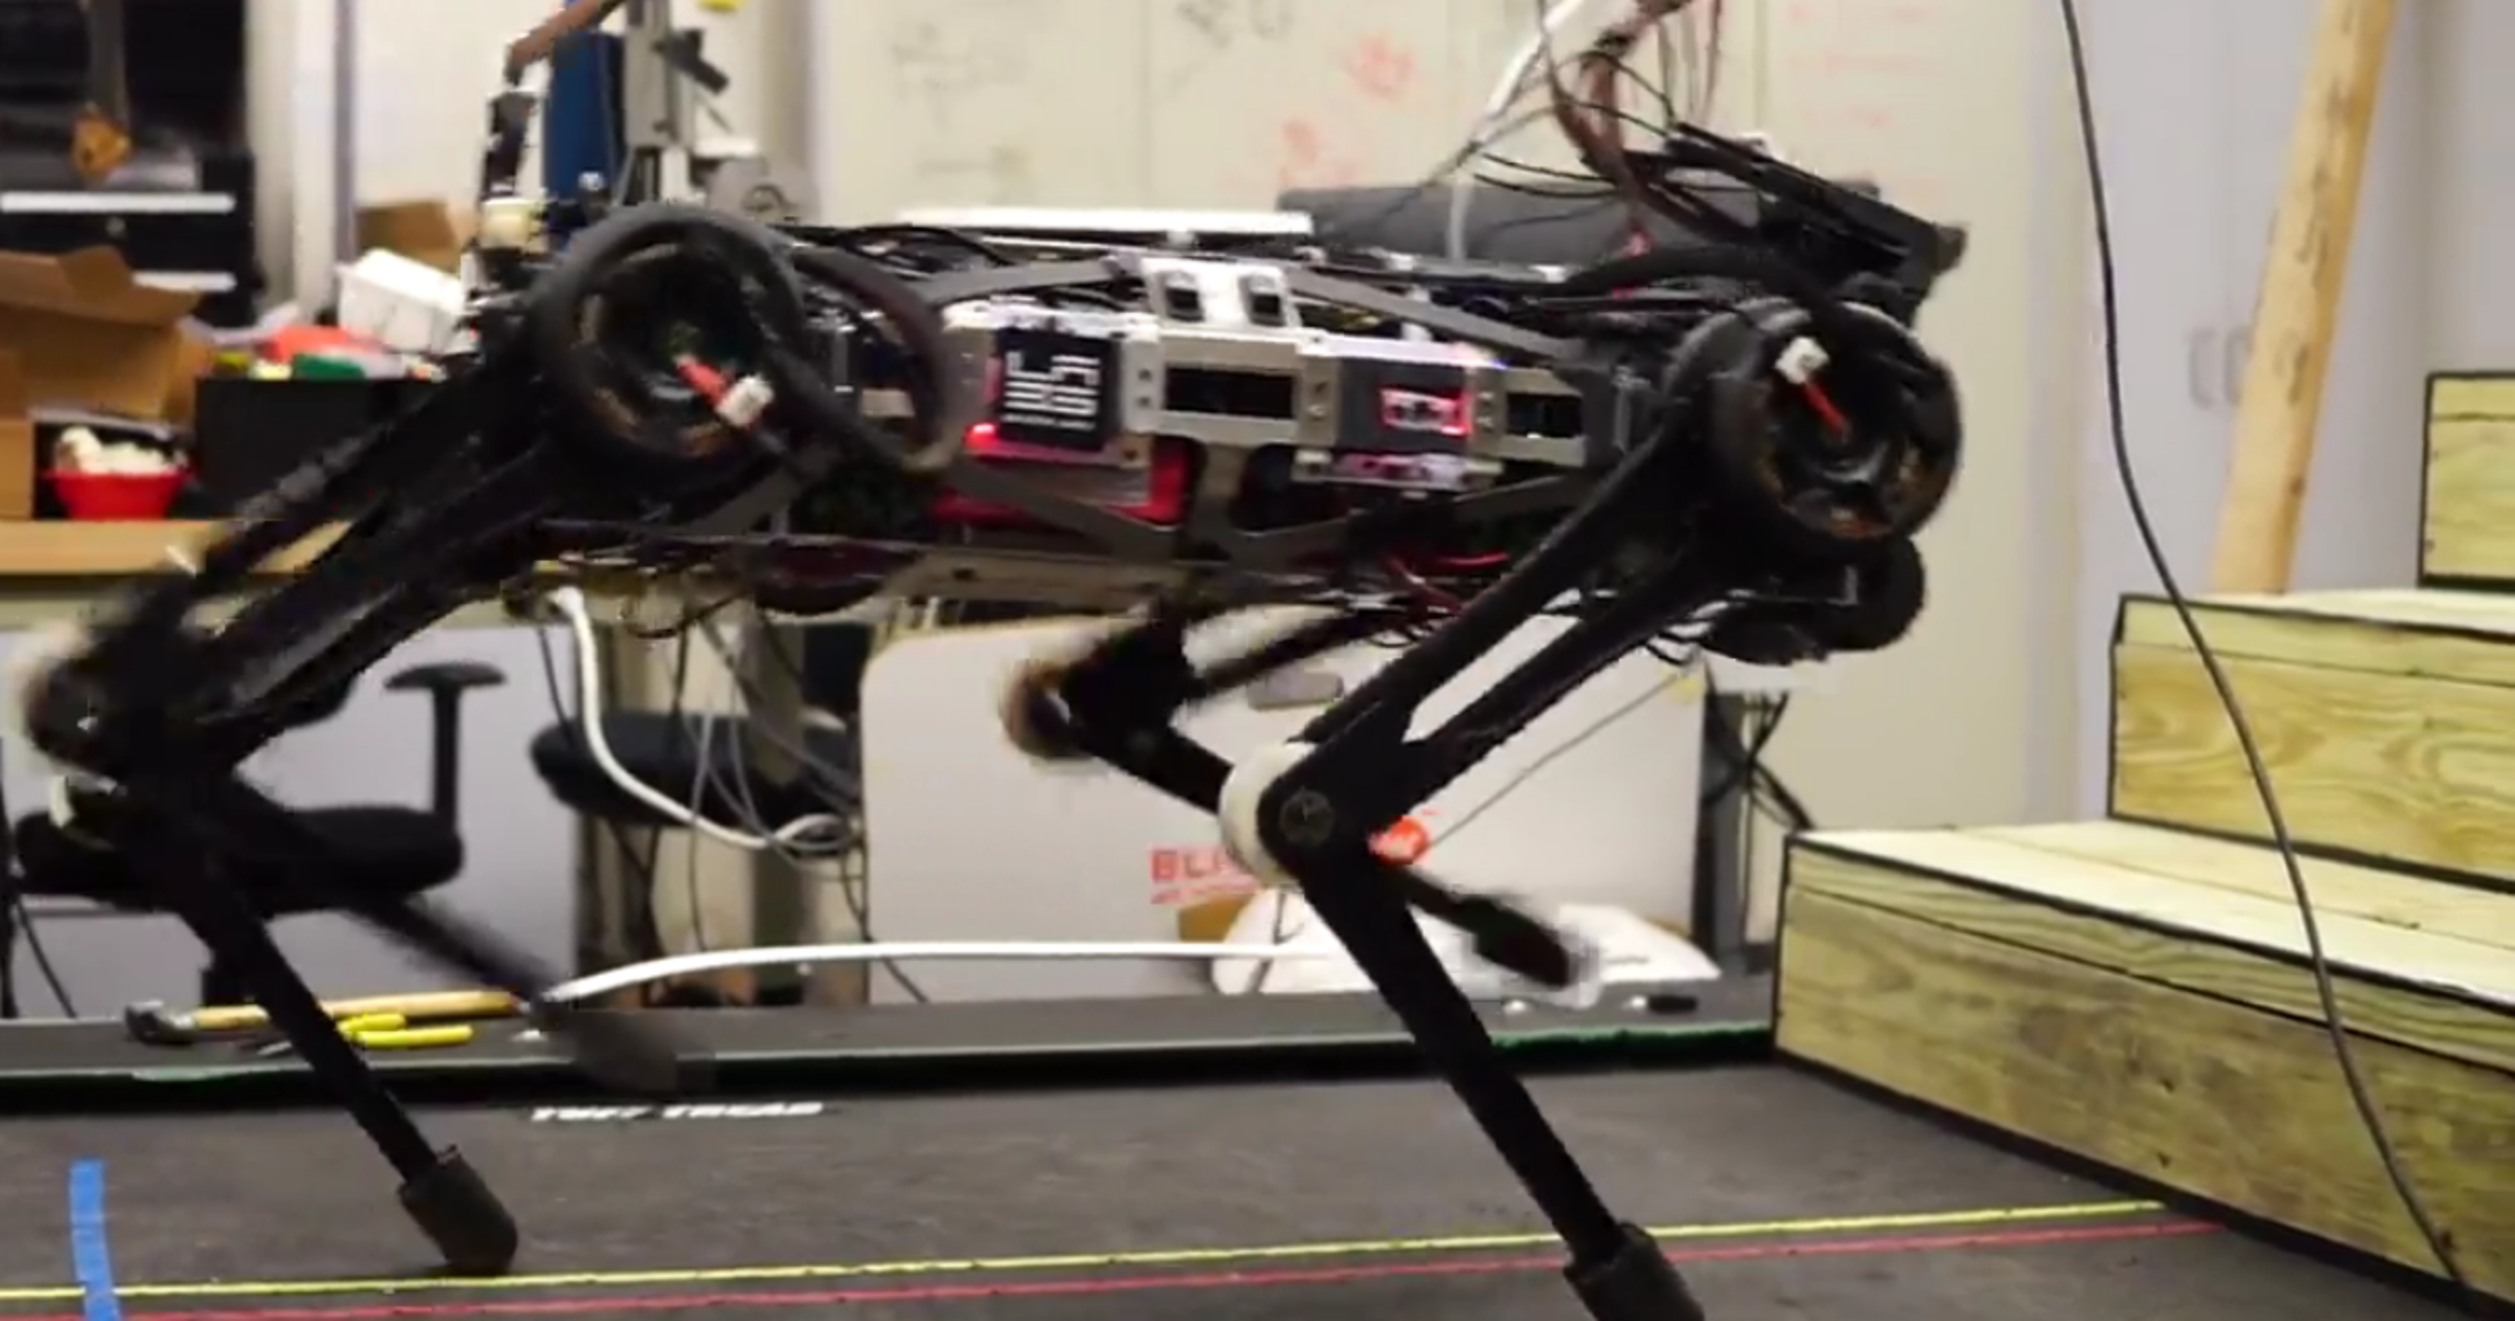
\includegraphics[width=\columnwidth]{Figures/RobotIntro.pdf}
\caption{A robust controller is used for general robot locomotion in unstructured terrains, but a method of external environment sensing is needed for the robot to know that its nominal foot swing trajectory will not be able to clear the stair obstacle.}
\label{fig:RI}
\end{figure}

Paper on creating the disparity map \cite{1467526} 



{\small
\bibliographystyle{ieee}
\bibliography{egbib}
}
%https://pdfs.semanticscholar.org/872e/9d71311cf9f00ec0ebc2c6b592c12a44d1f0.pdf

\end{document}
